\documentclass[11pt]{report}
\usepackage{graphicx}
\usepackage{float}
\title{EE314 Experiment 4 Elementary Gate Networks}
\date{2018\\ April}
\author{Nail Tosun - 2094563\\ Electric and Electronic Engineering Departmant, METU}
\begin{document}
\maketitle
2)
The F block must be 2x1 multiplexer. 
3)
74151 is an 8x1 multiplexer so that
\begin{figure}[H]
  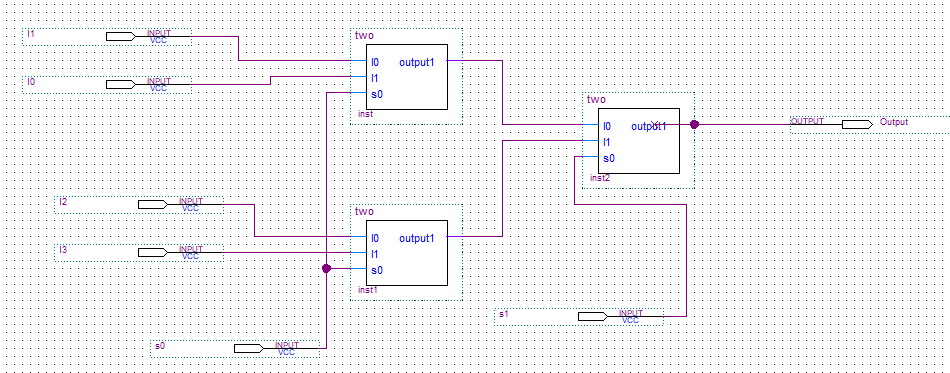
\includegraphics[width=\linewidth]{2x1}
  \caption{16 bit Multiplexer using 74151}
  \label{fig:zero}
\end{figure}  
4)
\begin{figure}[H]
  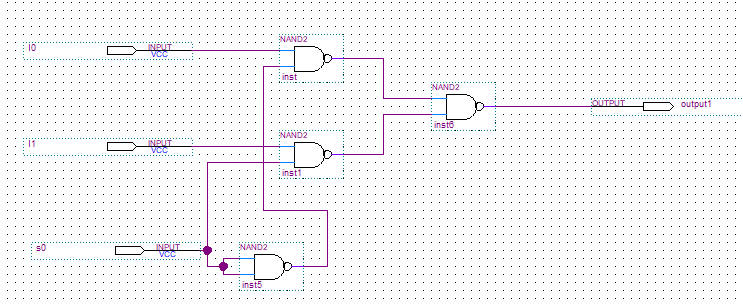
\includegraphics[width=\linewidth]{a}
  \caption{2x1 Multiplexer with NAND gates}
  \label{fig:zero}
\end{figure} 

\begin{figure}[H]
  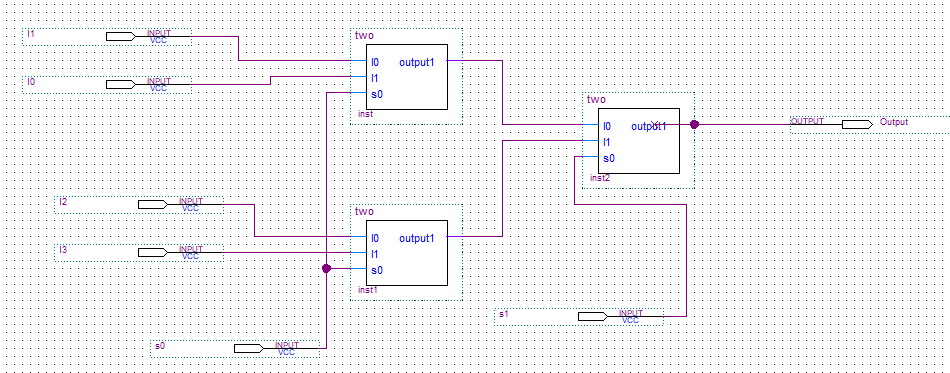
\includegraphics[width=\linewidth]{2x1}
  \caption{4x1 Multiplexer using 2x1 Multiplexer}
  \label{fig:zero}
\end{figure} 

\begin{figure}[H]
  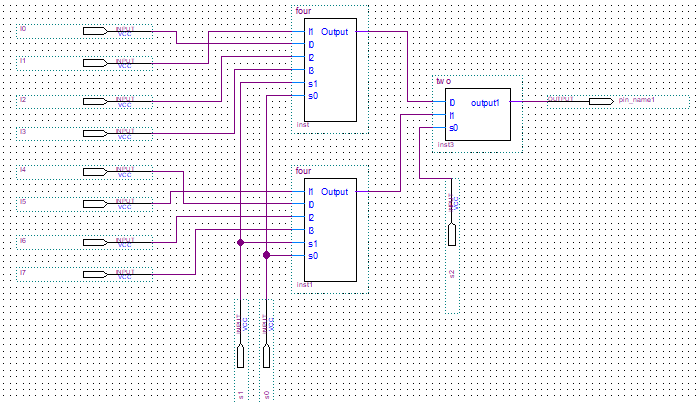
\includegraphics[width=\linewidth]{4x1}
  \caption{8x1 Multiplexer using 4x1 Multiplexer}
  \label{fig:zero}
\end{figure} 

\begin{figure}[H]
  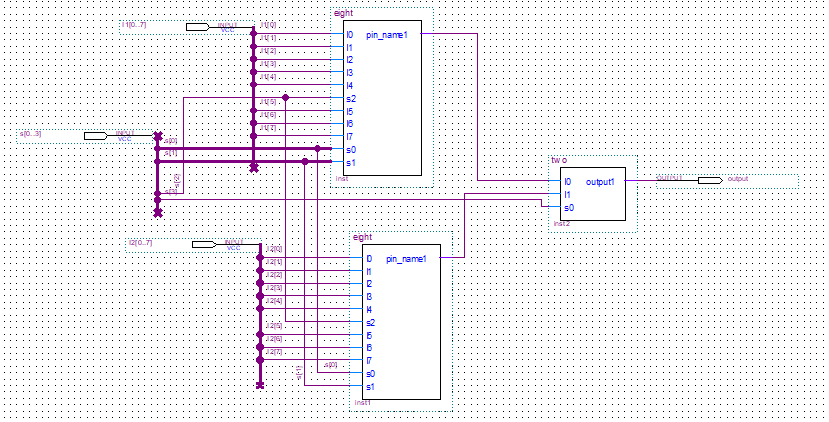
\includegraphics[width=\linewidth]{8x1}
  \caption{16x1 Multiplexer using 8x1 Multiplexer}
  \label{fig:zero}
\end{figure} 

\begin{figure}[H]
  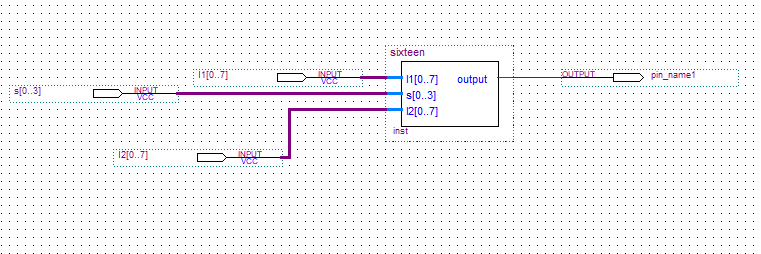
\includegraphics[width=\linewidth]{16x1}
  \caption{16x1 Multiplexer}
  \label{fig:zero}
\end{figure} 
5)
\begin{figure}[H]
  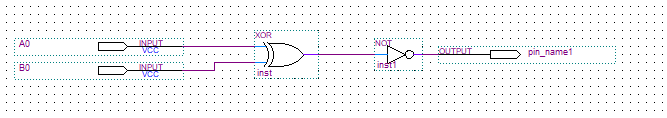
\includegraphics[width=\linewidth]{equal}
  \caption{Equivalence circuit using NAND}
  \label{fig:zero}
\end{figure} 

\begin{figure}[H]
  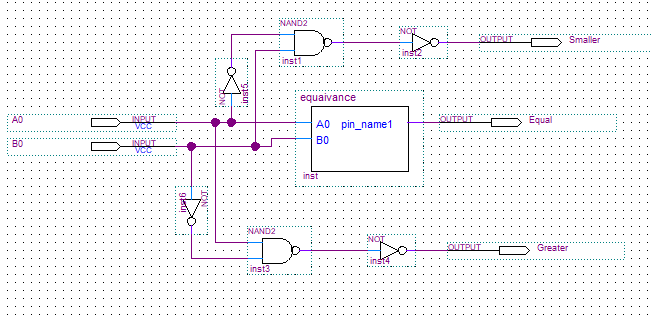
\includegraphics[width=\linewidth]{1bit}
  \caption{1 bit comparator}
  \label{fig:zero}
\end{figure} 

\begin{figure}[H]
  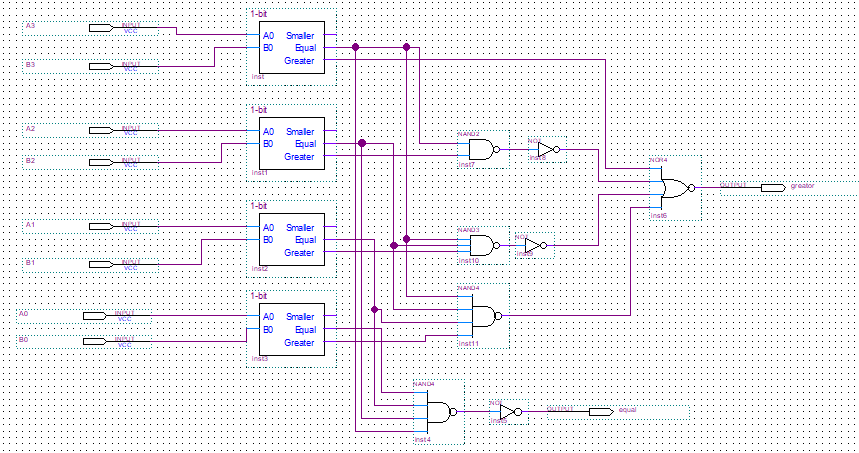
\includegraphics[width=\linewidth]{4bit1}
  \caption{4 bit comparator}
  \label{fig:zero}
\end{figure} 

\begin{figure}[H]
  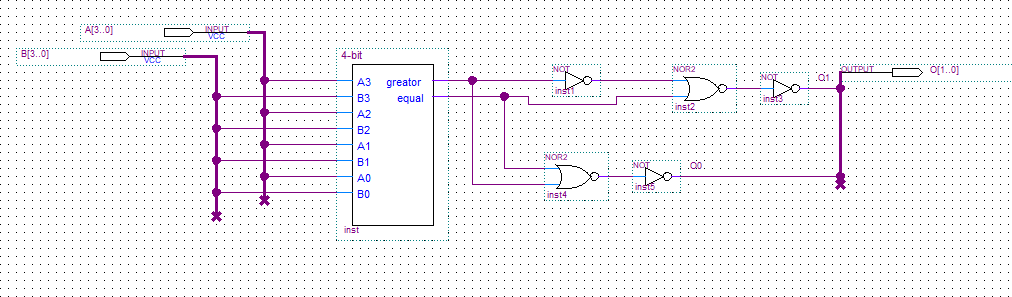
\includegraphics[width=\linewidth]{4bit}
  \caption{4 bit comparator}
  \label{fig:zero}
\end{figure} 

6)
\begin{figure}[H]
  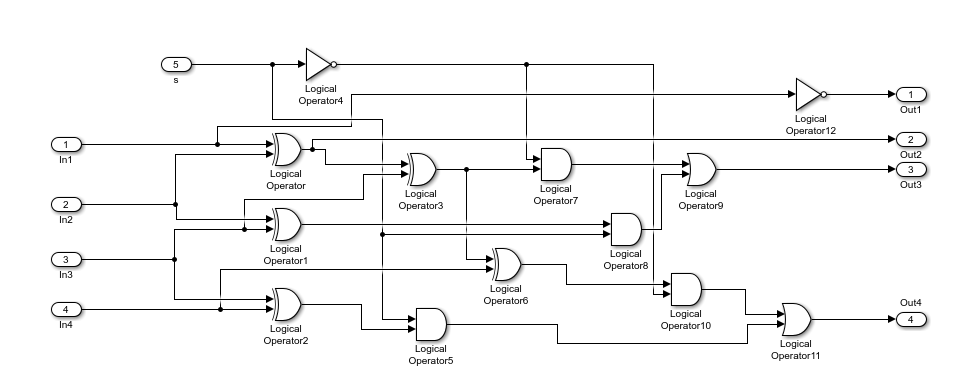
\includegraphics[width=\linewidth]{xor}
  \caption{gray code to binary and binary to gray code converter}
  \label{fig:zero}
\end{figure} 
\end{document}